\documentclass[12pt, titlepage=true, toc=bib]{scrartcl}


%Deutsche Silbentrennung
%Trennung von Wörtern mit Umlauten
%Deutsche Sprachregeln
\usepackage[utf8]{inputenc}
\usepackage[T1]{fontenc}
\usepackage[english]{babel}

%Schriftart
\usepackage[bitstream-charter]{mathdesign}
\usepackage[activate={true, nocompatibility}, final, tracking=true, kerning=true, spacing=true, factor=1100, stretch=10, shrink=10]{microtype}
%Selbe Schriftart für Überschriften												
\addtokomafont{disposition}{\normalfont\bfseries}

\usepackage{amsmath}

%Zeilenabstand							
\usepackage[onehalfspacing]{setspace}

%Literaturverwaltung
\usepackage[backend=biber, style=authoryear, date=year, doi=false, isbn=false, url=false, maxcitenames=2, maxbibnames=8]{biblatex}		
%Formatierung für Anführungszeichen
\usepackage[autostyle]{csquotes}
%u.a. in et al. umwandeln
\DefineBibliographyStrings{ngerman}{andothers = {{et\,al\adddot}},}
%Formatiert die Zitationsklammern
\renewcommand{\labelnamepunct}{\addcolon\addspace}
\renewcommand{\postnotedelim}{\addcolon\addspace}
\DeclareFieldFormat{postnote}{#1}
\DeclareFieldFormat{multipostnote}{#1}
%Leerzeile zwischen den Einträgen im Literaturverzeichnis
\setlength{\bibitemsep}{0.5\baselineskip plus 0.5\baselineskip}
%Schrägstrich bei zwei Autor*innen
\renewcommand{\multinamedelim}[0]{/}
\renewcommand{\finalnamedelim}[0]{/}
%URL bei Artikel- und Büchereinträgen entfernen
\DeclareSourcemap{
  \maps[datatype=bibtex]{
    \map{
      \pertype{article}
      \pertype{book}
       \step[fieldset=url, null]
    }
  }
}


\addbibresource{HA_SNA.bib}

%Seitenränder
%\usepackage[right=4	cm,]{geometry}

%Paket, um Grafiken einzubinden
\usepackage{graphicx}
%\usepackage{float}
%Paket, um Grafiken davon abzuhalten, außerhalb bestimmter grenzen zu floaten [section]: verbietet gleiten außerhalb der Section
%\usepackage[section]{placeins}
%zum Formatieren der Bildunterschriften
\usepackage{caption}
\captionsetup{format=plain, justification=justified, singlelinecheck=off, width=.95\linewidth,  font={small, singlespacing}}
%\captionsetup[table]{position=below}
\setkomafont{captionlabel}{\bfseries}

%Wird für das r-Paket stargazer benötigt
\usepackage{dcolumn}

%Listen
%\usepackage{enumitem}

%pdf-Dateien einbinden
%\usepackage{pdfpages}

%Anhang ohne Seitenzahl im ToC
%\makeatletter
%\let\partbackup\l@part
%\renewcommand*\l@part[2]{\partbackup{#1}{}}
%\makeatother

\clubpenalty = 10000
\widowpenalty = 10000
\displaywidowpenalty = 10000

%Verlinktes ToC
\usepackage[colorlinks, pdfpagelabels, pdfstartview=FitH, bookmarksopen=true, bookmarksnumbered=true, linkcolor=black, urlcolor=black, plainpages=false, hypertexnames=false, citecolor=black]{hyperref}



\begin{document}

\titlehead{\flushleft{University of Copenhagen\\
			Department of Political Science\\
			Social Network Analysis (ASTK18106U)\\
			Yevgeniy Golovchenko
			}}
\author{Ole Fechner, Johannes Kopf}
\title{Structure and Strategy of the Internet Research Agency on Twitter}


\date{\normalsize{Copenhagen, \today}}

\publishers{\flushleft{\normalsize{Boddinstr. 15\hfill Moselstr. 50\\
							 12053 Berlin\hfill 50674 Cologne\\
							 ole.fechner@fu-berlin.de\hfill jkopf@posteo.de\\
							 MA Political Science\hfill MA Political Science}}}

\maketitle[0]

\newpage

\thispagestyle{empty}
\tableofcontents

\newpage
\setcounter{page}{1}

\section{Introduction}

\section{Agenda-building and Astroturfing}

The process of trying to move an actors agenda to the agenda of other actor's, especially policymakers, is defined as \textit{agenda-building} (\cite[3]{linvill_troll_2018}). This can also be extended to the question of how the public views certain issues, usually by analyzing media coverage of those issues: ``Agenda-building research examines how certain groups, such as those in politics and business, influence what issues journalists cover as well as how the public views issues'' (\cite[434]{parmelee_agenda-building_2014}). Since the rise of social media platforms like Twitter and Facebook, agenda-building takes place in those environments. This is due to journalists drawing heavily on Twitter for their job and, on the other hand, research shows that Twitter is the most popular social media platform for participating in political discussions, which from there are often taken to other media (\cite[435, 437]{parmelee_agenda-building_2014}). Influencing the citizens of another country through the use of media is nothing new, rather it is regularity used in conflicts or during war. ``However, Russia's work on social media has taken agenda-building efforts by nations into a new context'' (\cite[3]{linvill_troll_2018}).

Closely linked to agenda-building is a second phenomenon called (political or/and online) \textit{astroturfing}, which can be characterized as the ``creation of a false or exaggerated impression of grassroots support'' (\cite{harcup_astroturfing_2014}). It describes the strategic and coordinated approach of a group with the aim to create the impression of a certain public opinion, that might not exist in that way. On social media, those groups use many different accounts that post and interact with regular users to create the desired impression. For the purpose of this paper, we see astroturfing as a strategy of agenda-building. The anonymity provided by platforms like Twitter, as well as the covert structure of those groups, make them very hard to discover (\cite[564]{yang_how_2017}). This exploratory study will therefore take the structure of the IRA as a staring point, instead of the presumed agenda behind the organization. Social network analysis, which will be introduced in the next section, offers an excellent tool box to conduct this task.


\section{Social Network Analysis of the IRA Retweet Network}

To analyze the structure and possible strategies of the IRA, we will take social network analysis (SNA) as the method of choice. The data-driven character of SNA -- the notion of people relating to each other, and the significance put into the structure and strength of those relations being almost the only one (\cite[982]{golovchenko_state_2018}) -- makes it especially viable for our exploratory approach. SNA conceptualizes the linkages between actors as \enquote{channels for transfer or \enquote{flow} of resources}, while the actors themselves are seen as ``interdependent rather than independent, autonomous units'' (\cite[4]{wasserman_social_1994}). Therefore, the different actor attributes are seen as emerging out of their relations and not vice versa, as in most other quantitative analyses (\cite[8]{wasserman_social_1994}). This allows us to ignore the question of the actual people behind different accounts and tell something about the IRA and its structure, as well as its strategy, as a whole. The most important relation to analyze how the IRA uses astroturfing as a strategy for agenda-building is the distribution of information, in this case via retweets. Accordingly, the foundation of this paper will be a social network consisting of Twitter accounts as nodes and retweets as edges (or linkages).


\subsection{Data: An Ego-Centered Retweet Network}

We will use a dataset, published by NBC News (\cite*{popken_twitter_2018}), consisting of 203,451 Tweets by 453 accounts between July 2014 and September 2017, which were linked to the IRA by an official document handed over to US Congress by Twitter. Twitter justifies this linking by referring to ``third party sources'', which makes it impossible to reconstruct or evaluate their method. Therefore, we have to assume those accounts' links to the IRA to be correct, as it is the best evaluation available.

To create the social network, we need to clean the data: First, we drop any of the tweets that are not retweets, which leaves us with 147,428 retweets by 453 troll accounts. Second, 120 trolls, who did not retweet at all, were dropped accordingly. Our dataset now consists a set of 333 unique troll Twitter handles\footnote{A Twitter handle is the screen name of a Twitter account that can be changed by the users.}, who are retweeting others. A variable stating the unique User ID is used to validate uniqueness of the users, showing that there are indeed no duplicate User IDs in the dataset. Since, we only have information about who these 333 accounts did retweet, but not by whom they were retweeted, the network is ego-centered around the group of 333 trolls. Of these 333 trolls, 151 (ca 45\%) retweeted others and were themselves retweeted by other trolls, thus being both sender and receiver. 182 (ca 55\%) trolls only retweeted others, but were not retweeted themselves, making them only senders.\footnote{We define a retweet sender as the person retweeting an original Tweet by another person, who, accordingly, is the retweet receiver.} A third group of 71 trolls was found by looking at who was retweeted by the original group of trolls in the data, thus increasing the number of trolls in our data to a group of 404. These 71 trolls were retweeted by others, though did not send retweets themselves. Finally, the big body of users in the dataset consists of 36,485 users, who are retweeted by the trolls, but are not themselves categorized as trolls by Twitter. Table~\ref{tab:userstat} gives a first overview over out dataset. Overall, there are 36,889 unique twitter users in the dataset, 404 classified trolls and 36,485 non-trolls. The retweets contain relational information about one user retweeting another, therefore creating a directional edge between the two. Thus, the graph is a directed, ego-centered network of 404 IRA accounts with 36,889 unique Twitter accounts as nodes and edges representing retweets from the sender to the receiver.


\begin{table}[!htbp] \centering 
\begin{tabular*}{.95\linewidth}{@{\extracolsep{\fill}} l r r r} 
\\[-1.8ex]\hline 
\hline \\[-1.8ex] 
User & N & Senders & Receivers \\ 
\hline \\[-1.8ex] 
Troll & 404 & 333 & 222 \\ 
Non-Troll & 36,485 & 0 & 36,485 \\ 
\hline \\[-1.8ex]
Total & 36,889 & 333 & 36,707 \\ 
\hline \\[-1.8ex] 
\end{tabular*} 
  \caption{User Statistics} 
  \label{tab:userstat}
\end{table} 


To further extend our data and our scope of analysis, we are adding additional qualitative information on the IRA trolls, provided by Darren Linvill and Patrick Lee Warren (\cite*{linvill_troll_2018}) via the online news outlet FiveThirtyEight (citation). Linvill and Warren conduct a qualitative analysis, categorizing a sample of 1,133 IRA troll accounts by examining the tweet content and the account names, applying a temporal analysis of the trolls tweeting behavior after. They ``identified five categories of IRA-associated Twitter handles, each with unique patterns of behaviors: \textit{Right Troll}, \textit{Left Troll}, \textit{Newsfeed}, \textit{Hashtag Gamer}, and \textit{Fearmonger}.'' (\cite[6]{linvill_troll_2018}). In addition, there are three categories, which are not used within their analysis, those being \textit{Non-English}, \textit{Commercial} and \textit{Unknown}. The categories \textit{Right Troll} and \textit{Left Troll} need little explanation, as they include users who broadcasted right-leaning populist and socially liberal messages. \textit{Hashtag Gamers} are users who are playing word games on Twitter, mostly non-political, though sometimes including left- or right-leaning messages. \textit{Newsfeed} Trolls are posing as local US News Agencies, mostly linking to legitimate news content, often with a pro-Russian perspective. Fearmongers spread news of crisis events such as Tweets about salmonella infections. The \textit{Non-English} troll category includes users who tweeted in other languages than English, predominately Russian, some German and little French and Spanish. \textit{Commercial} Trolls are not included in our dataset. Finally, users were categorized as \textit{Unknown}, if they could not be assigned to other categories for lack of information in their tweets. These categories will be included in this paper's analysis, since might be interesting to see how they interact with the other trolls. We are appending Linvill and Warren's account categories to our data, finding categories are available for 394 of the 404 troll handles in our dataset, meaning that around 98\% of the trolls in our dataset are categorized. Table~\ref{tab:trollstat} shows the distribution of the categories among our dataset.

\begin{table}[!htbp] \centering 
\begin{tabular*}{.95\textwidth}{@{\extracolsep{\fill}} l r r r r} 
\\[-1.8ex]\hline 
\hline \\[-1.8ex] 
Category & N & Senders & Receivers & Average\_Followers \\ 
\hline \\[-1.8ex] 
Right & 101 & 75 & 90 & 4649 \\ 
Left & 110 & 104 & 48 & 1783 \\ 
Hashtag Gamer & 61 & 43 & 60 & 3021 \\ 
Non-English & 106 & 100 & 7 & 2127 \\ 
Newsfeed & 11 & 1 & 10 & 16446 \\ 
Fearmonger & 4 & 0 & 4 & 0 \\ 
Unknown & 11 & 10 & 3 & 3306 \\ 
\hline \\[-1.8ex]
Total & 404 & 333 & 222 & 4476 \\ 
\hline \\[-1.8ex] 
\end{tabular*} 
 \caption{Troll Statistics} 
 \label{tab:trollstat} 
\end{table} 
 
As another attribute, we are appending information on the count of followers of the troll accounts from a second dataset provided by NBC news. The information on the count of followers provided only includes one figure and does not vary over time, without specification of when these follower counts were obtained. We will assume that they are at least to some degree representative and use them as a heuristic. Table~\ref{tab:trollstat} gives the average number of followers for each account category.

Lastly, we are using the full time period of retweets, from July 2014 to September 2017. This paper is not interested in a time period preceding a specific event, like an election or a specific trending discussion, but rather strategic behavior of the trolls in general. That is why it seems to be the right approach to include all of the Tweets in the analysis.

\subsection{Methods}

To understand the IRA's division of labor between the accounts, we begin with testing weather Linvill and Warren's qualitative findings of the different account types would be reproducible via using network properties. For this, we will draw on a community detection algorithm based on modularity, known as the Louvain Method (\cite{blondel_fast_2008}).\footnote{For our network, this algorithm produced the best results. The Infomap algorithm (\cite[cf.][]{rosvall_maps_2008}) results in one big community containing ca 98\% of the nodes.} Communities are mesoscopic structures of a graph, that consist ``of a group of nodes that are relatively densely connected to each other but sparsely connected to other dense groups in the network'' (\cite[1083]{porter_communities_2009}). The Louvain algorithm is based on modularity, ``a scalar value between -1 and 1 that measures the density of links inside communities as compared to links between communities'' (\cites[2]{blondel_fast_2008}[cf. also][1089]{porter_communities_2009}). It approximately maximizes the modularity for each node, thus identifying communities. Finally we will compare the communities with Linvill and Warren's account types, to see weather we can better understand the identified community structure.

One important measure for the cooperation of the accounts is graph density, the proportion of all possible edges that are present in the graph (\cite[101]{wasserman_social_1994}). Since the network is ego-centered, it only makes sense to calculate density for the troll subgraph. We will then compare densities of the different communities, which can give an indication weather the IRA has distinctive strategies for those groups. Following Wassermann and Faust (\cite*[102]{wasserman_social_1994}) we calculate the density of the different community subgraphs \( \Delta_{c} \) as: \[ \Delta_{c} = \frac{2L_{c}}{g_{c}(g_{c} - 1)} ,\] where \( L_{c} \) is the number of edges present in the community subgraph, and \( g_{s} \) is the number of nodes in said graph. In communities with higher density, the accounts are working more together, meaning they spread information further through retweeting, while accounts in less dense communities rely more on information they put into the network themselves.

Identifying the most important accounts helps to understand the structure of the IRA. Operationalizing importance in SNA is usually done through centrality and prestige indices, whereas not only the chosen actors are considered prestigious, but also those doing the choosing (\cite[170]{wasserman_social_1994}). Since the network is ego-centered around the troll accounts, the indices have limited reach in their interpretation, but still deliver important insights. To show the most central accounts, we will calculate outdegree. The index can only be computed for IRA accounts, since they are the only retweeting in our dataset. We will calculate the outdegree weighted and unweighted respectively, the former results in the accounts that retweet the majority of different accounts, the latter in those retweeting the most.\footnote{A weighted graph is a graph in which each edge carries a value (\cite[140]{wasserman_social_1994}), in this case the number of retweets between two accounts. In an unweighted graph, each edge has the value 1.} The outdegree of a node \( d_{out}(n_{i}) \) is computed as \[ d_{out}(n_{i}) = \sum_{j} x_{ij} ,\] where \( x_{ij} \) is an edge from \( i \) to \( j \) (\cite[cf.][178]{wasserman_social_1994}. For the weighted outdegree \( x_{ij} \) is multiplied by the value of the edge. Prestige, on the other hand, will be calculated through indegree, which results in those accounts retweeted the most and can therefore tell about what accounts the IRA draws on. It will also be computed for the weighted and unweighted graph separately, which shows the accounts retweeted by the majority of different accounts and those retweeted the most in general respectively. The indegree of a node \( d_{in}(n_{i}) \) is computed simply as \[ d_{in}(n_{i}) = \sum_{j} x_{ji} ,\] where \( x_{ji} \) is an edge from \( j \) to \( i \) (\cite[cf.][202]{wasserman_social_1994}. For the weighted outdegree \( x_{ji} \) is multiplied by the value of the edge.

Finally, we will look at the most engaged users in the network to identify the so-called super-spreaders of information. In SNA, the ability to spread information better than other individuals is ascribed to their unique location in the network, which makes identifying those a prime task of analyzing networks used for false information (\cite[1]{pei_searching_2015}). Pei et al. (\cite*{pei_searching_2015}) show that, compared to other approaches, the k-core method predicts the super-spreaders most accurately. \enquote{A k-core is a maximal subset of the network where all nodes are connected to at least \enquote{k} number of other nodes: so \enquote{k} can be any whole number} (\cite[983]{golovchenko_state_2018}). Hence, the k-core specifies a subgraph via the number of ties that must be present between nodes, it is based on the nodal degree. We can define a subgraph \( G_{s} \) as a k-core if \[ d_{s}(i) \geq k \text{ for all } n_{i} \in N_{s} ,\] where \( d_{s}(i) \) is the (in-)degree of node \( i \) and \( N_{s} \) the set of nodes in the subgraph (\cite[266]{wasserman_social_1994}). Once again, the network being ego-centered limits the validity of the results, since every non-troll in reality has a higher degree through retweets from other non-troll accounts and retweeting themselves. We can therefore only identify the most important IRA accounts regarding their own network. To account for this, we will also compute the k-in-core through the indegrees. The idea is that information from one account is spread quickly, if this account is retweeted a lot and the accounts retweeting it also get retweeted a lot.

\section{Analysis}

In the preceding chapter, the agenda and methods of our analysis have been introduced. In this chapter, we will present the results of these measurements. First, the results of the modularity community detection algorithm are illustrated and new communities are established, based on these findings. Secondly, graph densities are investigated for these communities.

We run a modularity-based community detection, following the Louvain Method (\cite{blondel_fast_2008}). Figure 1 shows the distribution of algorithm communities among the qualitative account categories created by Linvill/Warren (\cite*{linvill_troll_2018}). For further analysis, we want to rely on communities that were computed with the Louvain Method, since they originate from the structure of ties within our dataset and this appears to be more consistent with the overall method of SNA. To not exceed the scope of this paper, we narrow down our analysis by merging all minor communities below an arbitrary threshold size of 50, since they presumably bear more risk of yielding unrepresentative findings. We then apply the qualitative categorization to our newly distincted communities. In Figure 1, we see that some categories overlap strongly with distinct communities, whereas other categories show a rather mixed composition in our data. 94\% of the left troll category is captured with one community, which will be our new left troll community. The hashtager community is 90\% captured by one community, which will be our new hashtager troll community. 90\% of the right troll category consist of two major communities with shares of 52\% and 38\%, which we merge to one new right troll community. We justify this merger by arguing that these two communities could represent distinct right-wing groups underneath a general right-wing community (e.g. Conspiracy Theorist vs. Alt Right User). (\cite{kaiser_unite_2018}).  We argue, that for these categories, which are overlapping with at least 90\%, there is sufficient congruence to continue using the qualitative attributes. The non-english troll category consists of multiple communities, with a biggest community share of 27\%. Non of the non-english or other categories passes our threshold community size of 50, which leaves us with four distinct communities: \textit{Right Troll}, \textit{Left Troll}, \textit{Hashtager} and \textit{Other}. It is important to note, that by using this set of communities, we are treating some nodes as e.g. right trolls, even though they have been categorized as left trolls by Linvill/Warren (\cite*{linvill_troll_2018}). This bears the risk of having biased results. Though, with the given incongruence of the account categorization with our detected communities, having some potential bias appears inevitable. In Figure~\ref{fig:distcat}, the distribution of account categories among our new communities is depicted, which illustrates this potential bias.

\begin{figure}[!ht]
\centering
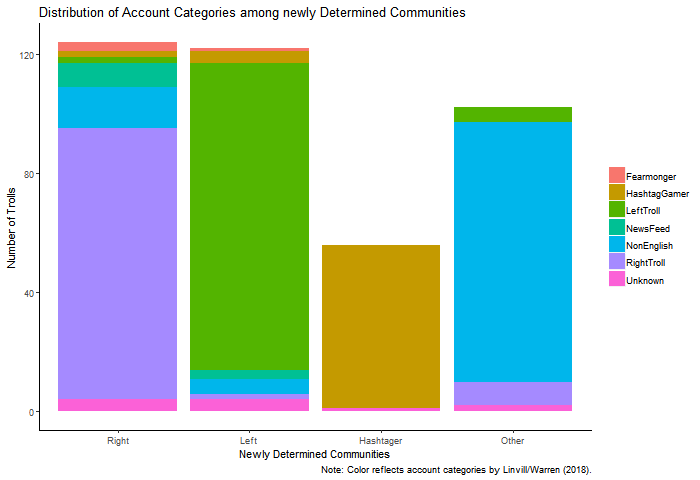
\includegraphics[width=0.95\linewidth]{figure2.png}% die Breite des eingefügten Bildes entspricht 95% einer Zeilenlänge
\caption{Distribution of account categories among communities detected by the Louvain Method. Color reflects account categories by Linvill/Warren}
\label{fig:distcat}
\end{figure}

Next, the graph densities are calculated for the subgraphs of our newly determined communities. Figure 3 shows the graph densities for the three communities for both directed and undirected versions of each subgraph. As a mode for creating an undirected graph from a directed one, we chose too keep a tie for every relationship that is only defined with a single directional tie, but also to collapse all reciprocal ties into one tie in the undirected graph. This avoids having multiple ties in one relationship. First of all, we see that the undirected subgraphs' densities are approximately twice as high as directed ones, with only minor deficits. With our mode of creating an undirected graph, we can interpret this that way, that there are not many reciprocal ties in the subgraphs. If there was a considerable amount of reciprocal ties, they would cause a higher density of the directed subgraph in comparison to the undirected one (>50\%).
%% hier figure3.png, title: "Graph Density for Community Subgraphs", Notes: evtl. Graph density formel nochmal
Examining the magnitude of densities across different community subgraphs, we find that the hashtager community is the most dense by a significant margin. Approximately 17.7\% of all possible ties are present for the undirected subgraph. This could relate to the nature of this community. As laid out above, hashtag gamers retweet themselves playing a word game, which means that it appears to consitute this community's cohesion to retweet one another frequently. Right trolls have the second largest density with 7.4\%, which is more than six times larger than the left community's density of 1.2\%, looking at the numbers for the undirected graphs.

We now want to analyse the degreeness of our graph. We start with the outdegree, which we use as a measure for centrality and the weighted outdegree, which gives addional information on the activity of the user. Because of our network is ego-centered around the central group of trolls, only troll accounts have outdegrees. Table~\ref{tab:out} shows the top 10 users ranked by outdegree.

\begin{table}[!htbp] \centering 
  \label{tab:out} 
\begin{tabular*}{.95\linewidth}{@{\extracolsep{\fill}} D{.}{.}{-3} D{.}{.}{-3} D{.}{.}{-3} D{.}{.}{-3} D{.}{.}{-3} D{.}{.}{-3} D{.}{.}{-3} } 
\\[-1.8ex]\hline 
\hline \\[-1.8ex] 
\multicolumn{1}{c}{User} & \multicolumn{1}{c}{Community} & \multicolumn{1}{c}{Category} & \multicolumn{1}{c}{Followers} & \multicolumn{1}{c}{Outdegree} & \multicolumn{1}{c}{Outdegree\_Weighted} \\ 
\hline \\[-1.8ex] 
\multicolumn{1}{c}{ameliebaldwin} & \multicolumn{1}{c}{Other} & \multicolumn{1}{c}{RightTroll} & 2,464 & 4,896 & 9,243 \\ 
\multicolumn{1}{c}{patriotblake} & \multicolumn{1}{c}{Other} & \multicolumn{1}{c}{RightTroll} & 2,035 & 2,856 & 4,106 \\ 
\multicolumn{1}{c}{hyddrox} & \multicolumn{1}{c}{Right} & \multicolumn{1}{c}{RightTroll} & 2,225 & 2,650 & 6,788 \\ 
\multicolumn{1}{c}{4} & \multicolumn{1}{c}{giselleevns} & \multicolumn{1}{c}{Hashtager} & \multicolumn{1}{c}{Unknown} & 24,344 & 2,282 & 5,403 \\ 
\multicolumn{1}{c}{5} & \multicolumn{1}{c}{cookncooks} & \multicolumn{1}{c}{Other} & \multicolumn{1}{c}{RightTroll} & 1,468 & 2,153 & 2,893 \\ 
\multicolumn{1}{c}{6} & \multicolumn{1}{c}{emileewaren} & \multicolumn{1}{c}{Other} & \multicolumn{1}{c}{RightTroll} & 1,909 & 2,116 & 2,891 \\ 
\multicolumn{1}{c}{7} & \multicolumn{1}{c}{dorothiebell} & \multicolumn{1}{c}{Right} & \multicolumn{1}{c}{RightTroll} & 1,893 & 2,010 & 2,874 \\ 
\multicolumn{1}{c}{8} & \multicolumn{1}{c}{baobaeham} & \multicolumn{1}{c}{Left} & \multicolumn{1}{c}{LeftTroll} & 1,032 & 1,802 & 3,215 \\ 
\multicolumn{1}{c}{9} & \multicolumn{1}{c}{michellearry} & \multicolumn{1}{c}{Right} & \multicolumn{1}{c}{RightTroll} & 3,229 & 1,611 & 2,677 \\ 
\multicolumn{1}{c}{10} & \multicolumn{1}{c}{\_nickluna\_} & \multicolumn{1}{c}{Right} & \multicolumn{1}{c}{RightTroll} & 1,457 & 1,597 & 2,825 \\ 
\hline \\[-1.8ex] 
\end{tabular*}
\caption{Top 10 Users ranked by Outdegree} 
\end{table} 

The first ranked user \textit{ameliebaldwin} really sticks out with an outdegree of 4,896, meaning that the user retweeted nearly 5,000 different users. The weighted outdegree of \textit{ameliebaldwin} is 9,243, which includes multiple retweets of the same user. Since the weighted outdegree is significantly higher than the unweighted one, this means that \textit{ameliebaldwin} retweeted a large number of users only a few times, rather than retweeting the same small number of users over and over again. The category and community allocation disagree for \textit{ameliebaldwin}. While the qualitative analysis by Linvill/Warren \cite*{linvill_troll_2018} found the user to be a right troll, the community detection algorithm did not find it to belong one of the major right troll communities. This exact pattern of disagreement reappears for three other users in Table 3. Subsequent to \textit{ameliebaldwin}, there is a group of accounts retweeting more than 2,000 different users, which is mainly dominated by right trolls following the categorization, but also with partial disagreement, following the above-mentioned pattern. The fourth ranked user \textit{giselleevns} sticks out for having the most followers in the ranking with 24,344. With a mean number of followers of 3,022 and a maximum of 61,109, \textit{giselleevns} appears to be one of the most followed accounts in the dataset. Though, it needs to be noted, that information on followers is only available for troll accounts in our dataset. Contrary to the mostly right troll dominated top ten ranked outdegree users, \textit{giselleevns} was allocated to the hashtager community, with disagreement of Linvill/Warren \cite*{linvill_troll_2018}, who could not attribute the account to a category. When ranking the account for weighted outdegree, as can be seen in Table~\ref{tab:wout}, the picture slightly changes. While some accounts like \textit{ameliebaldwin} and \textit{giselleevns} remain in high-ranked positions, six left troll accounts are now in the ranking, for which category and community allocation mostly agrees.

When examining the accounts with the highest indegrees, both trolls and regular accounts are included. We use indegree as a measure for prestige, as it shows how often a user is chosen to be retweeted by the trolls. Table 5 shows the ten highest ranked accounts for unweighted indegree. Here, mostly regular accounts are 

\begin{table}[!htbp] \centering 

  \label{tab:wout} 
\begin{tabular*}{.95\linewidth}{@{\extracolsep{\fill}} l r r r r r} 
\\[-1.8ex]\hline 
\hline \\[-1.8ex] 
\multicolumn{1}{c}{User} & \multicolumn{1}{c}{Community} & \multicolumn{1}{c}{Category} & \multicolumn{1}{c}{Followers} & \multicolumn{1}{c}{Outdegree} & \multicolumn{1}{c}{Outdegree weighted} \\ 
\hline \\[-1.8ex] 
\multicolumn{1}{c}{ameliebaldwin} & \multicolumn{1}{c}{Other} & \multicolumn{1}{c}{RightTroll} & 2,464 & 4,896 & 9,243 \\ 
\multicolumn{1}{c}{hyddrox} & \multicolumn{1}{c}{Right} & \multicolumn{1}{c}{RightTroll} & 2,225 & 2,650 & 6,788 \\ 
\multicolumn{1}{c}{giselleevns} & \multicolumn{1}{c}{Hashtager} & \multicolumn{1}{c}{Unknown} & 24,344 & 2,282 & 5,403 \\ 
\multicolumn{1}{c}{patriotblake} & \multicolumn{1}{c}{Other} & \multicolumn{1}{c}{RightTroll} & 2,035 & 2,856 & 4,106 \\ 
\multicolumn{1}{c}{mrclydepratt} & \multicolumn{1}{c}{Left} & \multicolumn{1}{c}{LeftTroll} & 914 & 1,583 & 3,262 \\ 
\multicolumn{1}{c}{brianaregland} & \multicolumn{1}{c}{Other} & \multicolumn{1}{c}{LeftTroll} & 768 & 1,360 & 3,259 \\ 
\multicolumn{1}{c}{baobaeham} & \multicolumn{1}{c}{Left} & \multicolumn{1}{c}{LeftTroll} & 1,032 & 1,802 & 3,215 \\ 
\multicolumn{1}{c}{datwisenigga} & \multicolumn{1}{c}{Left} & \multicolumn{1}{c}{LeftTroll} & 904 & 1,540 & 3,196 \\ 
\multicolumn{1}{c}{willisbonnerr} & \multicolumn{1}{c}{Left} & \multicolumn{1}{c}{LeftTroll} & 571 & 1,563 & 3,155 \\ 
\multicolumn{1}{c}{melanymelanin} & \multicolumn{1}{c}{Left} & \multicolumn{1}{c}{LeftTroll} & 963 & 1,079 & 3,071 \\ 
\hline \\[-1.8ex] 
\end{tabular*} 
  \caption{Top 10 users ranked by weighted outdegree.} 
\end{table} 

The highest ranked left troll account \textit{mrclydepratt} has a weighted outdegree of 3,262 and an unweighted one of 914. Compared to the top ranked presumably right troll accounts, the left troll accounts approximately only have a maximum of half of the unweighted outdegree, but are much closer on the wheighted outdegree. This means that the left trolls retweet a smaller number of accounts more often than right trolls do. This relates to the lower graph density for the left troll community that was computed above.

\section{Discussion}

\section{Conclusion}

\section{Code (not included in word count)}



\newpage

\printbibliography


\end{document}
